% introduction au cours de C++

\subsection{Pourquoi C++ dans l'option RV ?}

\begin{frame}{Qu'est-ce que C++ ?}
\begin{figure}[htbp]
\begin{center}
   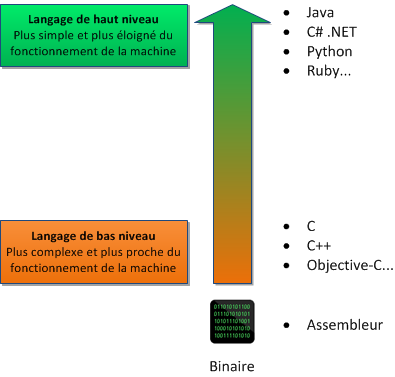
\includegraphics[scale=0.6]{fig/langages.png}
   \caption{(c) OpenClassrooms}
\end{center}
\end{figure}
\end{frame}

\subsection{Historique}

\begin{frame}{Histoire}
\begin{itemize}
\item 1958 : Algol
\item années 60 : CPL, puis BPCL puis B
\item 1970 : langage C (Dennis Ritchie 1969-1973)
\item 1979 : \textit{C with classes}
\item 1983 : C++ (amélioration du C ) : Bjarne Stroustrup
\item 1989 : C++ 2.0 (héritage multiple, classes abstraites)
\item 1995 : java
\item 1998 : début de la normalisation de C++ (inclusion de la \textit{SL})
\item 2011 : \textbf{C++11 devient un standard ISO}
\item 2014 : nouvelle norme C++14
\item 2017 : c++17 : définition figée en avril 2017, acceptation ISO/ANSI
\item 2020 : c++20 : à venir...
\end{itemize}
\end{frame}

\subsection{Organisation du cours}

\begin{frame}{Organisation}
\begin{itemize}
\item Peu de cours, beaucoup de pratique
\item un DS sur table à la fin (évaluation individuelle)
\item Base de travail
\begin{itemize}
\item Norme "C++11-14"
\item Utilisation de la machine virtuelle Linux installée en B114
\item outils : make, gcc
\item IDE ou éditeurs de texte : à votre convenance
\begin{alertblock}{Avertissement}
Vous pouvez utiliser d'autres outils (compilateurs), mais à vos risques et périls !
\end{alertblock}
\end{itemize}
\end{itemize}
\end{frame}
